\documentclass[../main.tex]{subfiles}

\graphicspath{{\subfix{../imgs/}}}

\begin{document}

\section{Operational Transconductance Amplifier}

In this project we will design an Operation Transconductance Amplifier (OTA) based on the neural amplifier from \textit{Harrison}\cite{harrison}.

\subsection{Introduction}

The OTA is a basic building block in analog design and finds a wide range of uses. The circuit topology we're using is a three current-mirror OTA. The amplifier takes in a balanced signal and has a single-ended output.

\begin{figure}[h]
    \centering
    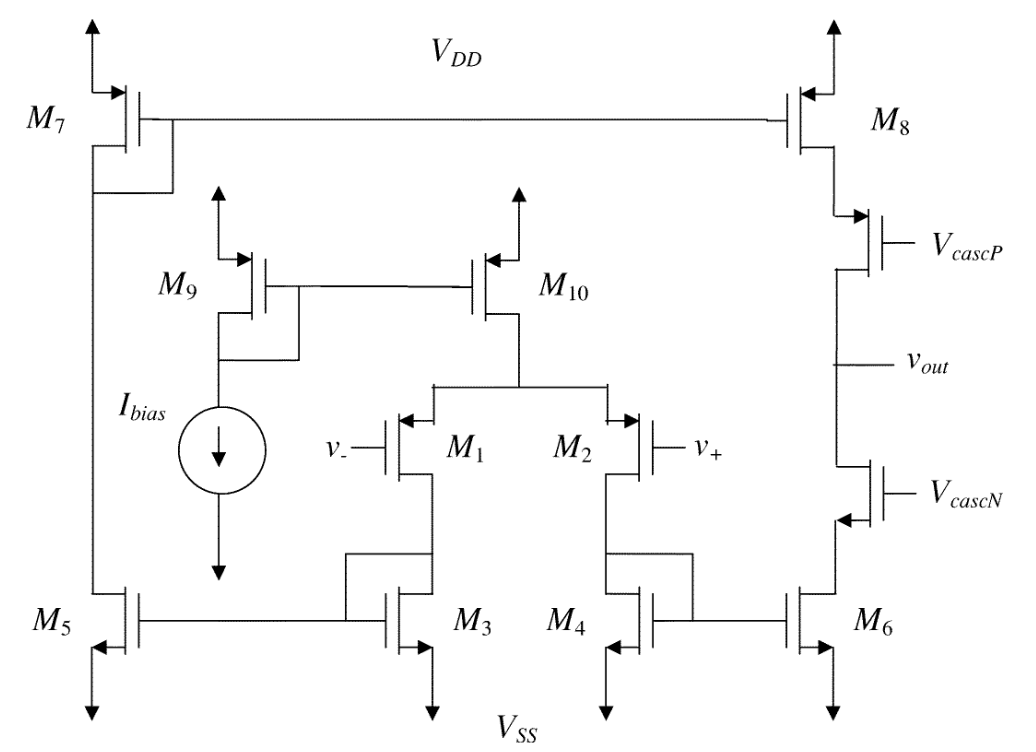
\includegraphics[width=0.5\textwidth]{harrison_schematic.png}
\end{figure}

Before starting circuit analysis we will quickly review performance targets

\begin{displaymath}
    \begin{array}{l l}
        \hline
        \text{Power Supply} & 1.2 \si{V} \\
        \hline
        \text{Power Consumption} & < 1 \si{\mu W} \\
        \text{Gain} & 40 \si{dB} \\
        \text{Output Voltage Range} & 1 \si{V} \\
        \text{CMRR} & 70 \si{dB} \\
        \text{PSRR} & 70 \si{dB} \\
        \text{Input-Referred Noise} & < 5 \si{\mu V (RMS)} \\
        \hline
    \end{array}
\end{displaymath}

\subsection{Analysis}

The input stage consists a long-tailed pair biased by current source $M_{10}$. The input voltages $V_+$ and $V_-$ are converted to currents by the input transistors transconductance $g_{m,1}$. This current is then mirrored by $M_{3,4}$ with ratio $1:B$. The upper PMOS current mirror has ratio $1:1$ for balance. \vspace*{10pt}

\noindent
Due to the mirroring, the total transconductance of the OTA

$$
G_M = B g_{m,1}
$$

\noindent
The output resistance of output stage is denoted $R_{out}$, the total voltage gain 

$$
A_V = G_M R_{out}
$$

\noindent
With a load $C_L$ the dominant pole

$$
\omega_{p} = \frac{1}{C_L R_{out}}
$$

\noindent
The gain-bandwidth product and slew rate

$$ \text{GBW} = \frac{G_M}{C_L}, \hspace*{20pt} \text{Slew Rate} = \frac{B I_{tail}}{C_L} $$


\subsection{Sizing}

\subsection{Simulation}

\subsection{Conclusion}


\end{document}